\section{Mod\`ele du Robot}
\label{sec:section1}

\subsection{Robot}
Chacun des bras du robot peuvent \^etre consid\'er\'es comme des robots s\'eriels ind\'ependants \`a six degr\'es de libert\'e.
On peut d'\'ecrire ce bras sous la forme suivante.
$$T_x(L_1) . R_y(\theta_1) . R_x(\theta_2) . T_y(L_2) . R_x(\theta_3) . T_y(L_3) . R_x(\theta_4) . T_x(-L_4) . R_z(\theta_5) . T_y(L_5) . R_y(\theta_6)$$

Les notations utilis\'ees seront les suivantes :
\begin{center}
  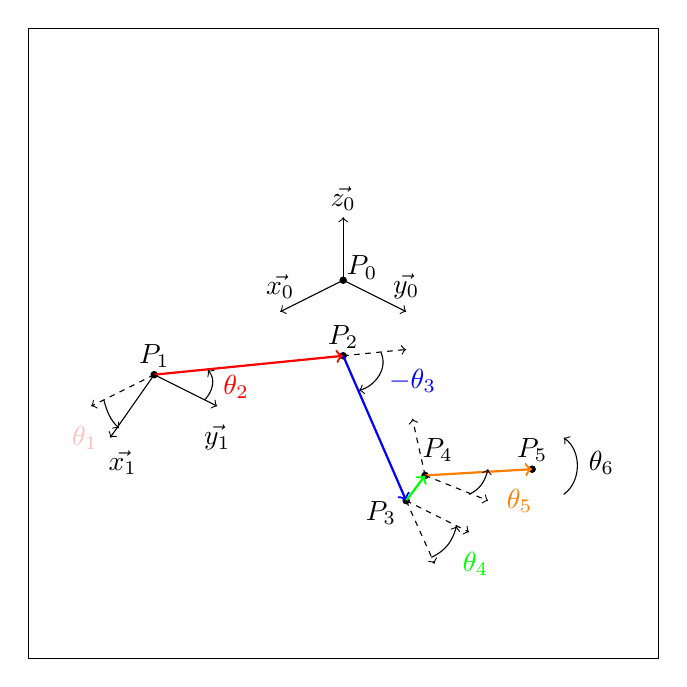
\begin{tikzpicture}[scale=0.8]
     \draw(0,0) -- (10,0) -- (10,10) --(0,10) -- (0,0);
     \draw[->] (5,6) -- (4,5.5);
     \draw[->] (5,6) -- (6,5.5);
     \draw[->] (5,6) -- (5,7);
     \draw (4,5.9) node {$\vec{x_0}$};
     \draw (6,5.9) node {$\vec{y_0}$};
     \draw (5,7.3) node {$\vec{z_0}$};

     \filldraw (5,6) circle (0.5mm);
     \draw (5.3,6.2) node {$P_0$};
     \filldraw (2,4.5) circle (0.5mm);
     \draw (2,4.8) node {$P_1$};
     \filldraw (5,4.8) circle (0.5mm);
     \draw (5,5.1) node {$P_2$};
     \filldraw (6,2.5) circle (0.5mm);
     \draw (5.6,2.3) node {$P_3$};
     \filldraw (6.3,2.9) circle (0.5mm);
     \draw (6.5,3.3) node {$P_4$};
     \filldraw (8,3) circle (0.5mm);
     \draw (8,3.3) node {$P_5$};

     \draw[thick,->,red] (2,4.5) -- (5,4.8);
     \draw[thick,->,blue] (5,4.8) -- (6,2.5);
     \draw[thick,->,green] (6,2.5) -- (6.3,2.9);
     \draw[thick,->,orange] (6.3,2.9) -- (8,3);

     \draw[->,dash pattern= on 2pt off 2pt] (2,4.5) -- (1,4);
     \draw[->] (2,4.5) -- (1.3,3.5);
     \draw (1.5,3.1) node {$\vec{x_1}$};
     \draw[->] (1.2,4.1) to[out=-75,in=135] (1.44,3.65);
     \draw[pink] (0.9,3.5) node {$\theta_1$};

     \draw[->] (2,4.5) -- (3,4);
     \draw (3,3.5) node {$\vec{y_1}$};
     \draw[->] (2.8,4.1) to[out=45,in=-45] (2.85,4.57);
     \draw[red] (3.3,4.3) node {$\theta_2$};

     \draw[->,dash pattern= on 2pt off 2pt] (5,4.8) -- (6,4.9);
     \draw[->] (5.6,4.85) to[out=-65,in=15] (5.25,4.25);
     \draw[blue] (6.1,4.4) node {$-\theta_3$};

     \draw[->,dash pattern= on 2pt off 2pt] (6,2.5) -- (6.45,1.5);
     \draw[->,dash pattern= on 2pt off 2pt] (6,2.5) -- (7,2);
     \draw[->] (6.4,1.6) to[out=25,in=-105] (6.8,2.1);
     \draw[green] (7.1,1.5) node {$\theta_4$};

    
     \draw[->,dash pattern= on 2pt off 2pt] (6.3,2.9) -- (7.3,2.5);
     \draw[->,dash pattern= on 2pt off 2pt] (6.3,2.9) -- (6.1,3.8);
     \draw[->] (7,2.6) to[out=25,in=-105] (7.3,3);
     \draw[orange] (7.8,2.5) node {$\theta_5$};

     \draw[->] (8.5,2.6) to[out=35,in=-35] (8.5,3.5);
     \draw (9.1,3.1) node {$\theta_6$};

  \end{tikzpicture}
\end{center}

\begin{center}
  \begin{tabular}{c @{~=~} c @{~=~} c}
    %\hline
    ||$\overrightarrow{P_0P_1}$|| & $L_1$ & $260~mm$ \\
    ||$\overrightarrow{P_1P_2}$|| & $L_2$ & $300~mm$ \\
    ||$\overrightarrow{P_2P_3}$|| & $L_3$ & $300~mm$ \\
    ||$\overrightarrow{P_3P_4}$|| & $L_4$ & $30~mm$ \\
    ||$\overrightarrow{P_4P_5}$|| & $L_5$ & $250~mm$ \\
    %\hline
  \end{tabular}
\end{center}

Notre objectif est de retrouver les valeurs articulaires du bras connaissant la position finale de l'effecteur.\\
\textbf{Input : } $(x, y, z, \phi, \theta, \psi)$\\
\textbf{Output : } $(\theta_1, \theta_2, \theta_3, \theta_4, \theta_5, \theta_6)$
\newpage

\subsection{G\'eom\'etrie Inverse}
\label{sub:geominv}

Nous allons utiliser une m\'ethode point-par-point afin de retrouver ces positions.
En partant du point $P_5$, nous pouvons calculer la position du point $P_4$ en utilisant les rotations $\phi$, $\theta$ et $\psi$ ainsi que le segment $L_5$.

\begin{equation}
\left( \begin{array}{c}X_4\\Y_4\\Z_4 \end{array} \right) 
= 
\left ( \begin{array}{c}
X_5 + sin(\psi) . cos(\theta) . L_5\\
Y_5 - (cos(\phi) . cos(\psi) . L_5 - sin(\phi) . sin(\psi) . sin(\theta) . L_5)\\
Z_5 - (cos(\phi) . sin(\psi) . sin(\theta) . L_5 + sin(\phi) . cos(\psi) . L_5)
\end{array} \right )
\end{equation}\\

Nous savons que le point $P_3$ est à une distance de $30~mm$ du point $P_4$.
De plus, la configuration du robot impose que $\overrightarrow{P_3P_4}$ soit parall\`ele au vector $\vec{x_0}$.
Donc la projection du point $P_3$ sur le plan $(O,\vec{x_0},\vec{z_0})$ doit se trouver sur un cercle autour de la projection du point $P_4$.

La projection de $P_3$ peut seulement se d\'eplacer sur une ligne d\'ependant uniquement du param\`etre $\theta_1$.
Nous pouvons donc calculer deux solutions possibles pour $\theta_1$ en d\'eterminant les deux tangentes au cercle passant par $P_1$ comme sur le sch\'ema suivant.

\begin{center}
  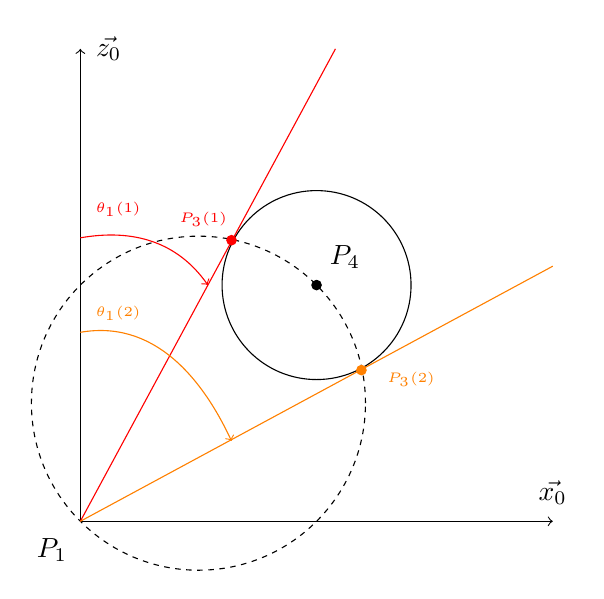
\begin{tikzpicture}[scale=1.2]
    \draw[->] (0,0) -- (5,0);
    \draw (5,0.3) node {$\vec{x_0}$};
    \draw[->] (0,0) -- (0,5);
    \draw (0.3,5) node {$\vec{z_0}$};

    \draw (-0.3,-0.3) node {${P_1}$};

    \filldraw (2.5,2.5) circle (0.5mm);
    \draw (2.8,2.8) node {$P_4$};
    \draw (2.5,2.5) circle (1cm);
    \draw[dash pattern = on 2pt off 2pt] (1.25,1.25) circle (1.7677cm);
    \draw[red] (0,0) -- (2.7,5); 
    \draw[orange] (0,0) -- (5,2.7);

    \filldraw[red] (1.6,2.975) circle (0.5mm);
    \filldraw[orange] (2.975,1.6) circle (0.5mm);
    \draw[red] (1.3,3.2) node {\tiny{$P_3(1)$}};
    \draw[orange] (3.5,1.5) node {\tiny{$P_3(2)$}};

    \draw[->,red] (0,3) to[out=10,in=125] (1.35,2.5);
    \draw[->,orange] (0,2) to[out=10,in=115] (1.6,0.85);
    \draw[red] (0.4,3.3) node {\tiny{$\theta_1(1)$}};  
    \draw[orange] (0.4,2.2) node {\tiny{$\theta_1(2)$}};
  \end{tikzpicture}
\end{center}

Connaissant $\theta_1$, nous pouvons calculer la position de $P_3$.
\saut\\
Soit, $\vec{v_1} = (-cos(\theta_1),0,sin(\theta_1))$,

\begin{equation}
\left( \begin{array}{c}X_3\\Y_3\\Z_3 \end{array} \right) 
= 
\left ( \begin{array}{c}
X_4 - L_4.\overrightarrow{v_{1x}}\\
Y_4 - L_4.\overrightarrow{v_{1y}}\\
Z_4 - L_4.\overrightarrow{v_{1z}}
\end{array} \right )
\end{equation}

Nous devons maintenant d\'eterminer $\theta_3$ et $\theta_2$.\\
Soit $D$ la distance entre $P_1$ et $P_3$, 

$$ D = \| \overrightarrow{P_1P_3}\|$$
Nous avons, $\alpha = \widehat{P_1P_2P_3}$ :
$$ \alpha = acos \left( \frac{L_2^2 + L_3^2 - D^2}{2.L_2.L_3} \right)$$
Si $L_2=L_3$, nous pouvons simplifier :
$$ \alpha = acos \left( 1 - \frac{D^2}{2.L_2^2} \right) $$
Alors,
$$ \theta_3 = \pi - \alpha $$
Pour $\theta_2$, nous pouvons utiliser la r\`egle des sinus ($\beta = \widehat{P_2P_1P_3}$) :
$$\beta = asin \left( \frac{L_3.sin(\alpha)}{D} \right) $$
Si $L_2=L_3$, nous pouvons simplifier :
$$\beta = \frac{\pi - \alpha}{2}$$
Alors
$$ \theta_2 = atan2( \sqrt{ (X_3 - X_1)^2 + (Z_3 - Z_1)^2}~,~(Y_3 - Y_1) ) - \beta$$
Sachant que $Y_1 = Z_1 = 0$, nous avons :
$$ \theta_2 = atan2( \sqrt{ (X_3 - X_1)^2 + Z_3 ^2}~,~Y_3 ) - \beta$$
\begin{equation}
\left( \begin{array}{c}X_2\\Y_2\\Z_2 \end{array} \right) 
= 
\left ( \begin{array}{c}
sin(\theta_1).sin(\theta_2).L_2 + L_1\\
cos(\theta_2).L2\\
cos(\theta_1).sin(\theta_2).L_2
\end{array} \right )
\end{equation}


\noindent 
Nous pouvons alors avoir $\theta_4$, 
$$\theta_4 = \frac{\pi}{2} - acos( \frac{\overrightarrow{P_2P_3}.(\overrightarrow{P_4P_5} \times \vec{v_1})}{\|\vec{A}\|.\|\overrightarrow{P_4P_5} \times \vec{v_1}\|} )$$
Et $\theta_5$, 
$$\theta_5 = \frac{\pi}{2} - acos( \frac{\overrightarrow{P_4P_5}.\vec{v_1}}{\|\overrightarrow{P_4P_5}\|.\|\vec{v_1}\|})$$
Nous pouvons calculer la g\'eom\'etrie inverse pour trouver le vecteur de rotation $\vec{y}$ en posant $\theta_6 = 0$ :
%We can compute the forward kinematics to find the rotation angle around $\vec{y}$ assuming $\theta_6 = 0$ :
\begin{small}
$$\gamma = atan \left( \frac{(c2 . (c3 . c4 . s1 - s1 . s3 . s4) - c3 . s1 . s2 . s4 - c4 . s1 . s2 . s3)}{(c2 . (c3 . s1 . s4 . s5 + c4 . s1 . s3 . s5) - s1 . s2 . s3 . s4 . s5 + c3 . c4 . s1 . s2 . s5 + c1 . c5)}\right)$$
\end{small}
Alors,
$$ \theta_6 = \theta - \gamma$$

%With this type of calculation we can not choose between two different solutions. On the other hand, the approximations made in the inverse trigonometric functions may return false results close to the singular positions.
Avec ce type de calculs nous ne pouvons pas choisir entre deux solutions. D'autre part, l'utilisation de fonctions trigonom\'etriques inverses peuvent donner des r\'esultats incoh\'erents proche des positions singuli\`eres.
\saut

Les tests donnent des r\'esultats satisfaisants en position avec une erreur inf\'erieur au dixi\`eme de millim\`etre quand la position est accessible.
Cependant pour les rotations l'erreur peut monter jusqu'\`a 5~degr\'es dans les cas susmentionn\'es.
